% Source: graduate-coursework/Sp26/CSCE763/Course_Assignments/HW3/HW3_CSCE_763.tex

\documentclass[border=4pt]{standalone}
\usepackage{amsmath}
\usepackage{amssymb}
\usepackage{graphicx}
\usepackage{tikz}
\usepackage{xcolor}
\usetikzlibrary{shapes.geometric, arrows.meta, positioning, patterns}

\definecolor{USC_Garnet}{HTML}{73000A}
\definecolor{USC_Sandstorm}{HTML}{FFF2E3}
\definecolor{USC_Black90}{HTML}{363636}
\definecolor{USC_Black70}{HTML}{5C5C5C}
\definecolor{USC_Black50}{HTML}{A2A2A2}
\definecolor{USC_Black10}{HTML}{ECECEC}
\definecolor{USC_Honeycomb}{HTML}{65780B}
\definecolor{USC_Atlantic}{HTML}{466A9F}
\definecolor{USC_Congaree}{HTML}{1F414D}
\definecolor{USC_Rose}{HTML}{CC2E40}
\definecolor{outputbg}{RGB}{245,245,245}
\definecolor{tealfill}{HTML}{00B8A9}
\definecolor{teallight}{HTML}{D4F0ED}
\definecolor{lightblue}{HTML}{D6EAF8}

\begin{document}
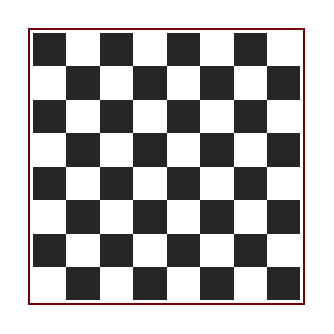
\begin{tikzpicture}
  \draw[thick, USC_Garnet] (0,0) rectangle (3.5,3.5);
  \foreach \i in {0,...,7} {
    \foreach \j in {0,...,7} {
      \pgfmathtruncatemacro{\checkcolor}{mod(\i+\j,2)}
      \ifnum\checkcolor=0
        \fill[white] ({0.05+\i*0.425}, {0.05+\j*0.425}) rectangle ({0.05+\i*0.425+0.425}, {0.05+\j*0.425+0.425});
      \else
        \fill[black!85] ({0.05+\i*0.425}, {0.05+\j*0.425}) rectangle ({0.05+\i*0.425+0.425}, {0.05+\j*0.425+0.425});
      \fi
    }
  }
\end{tikzpicture}
\end{document}
